% Chapter Template

\chapter{Option Pricing And Deep Learning} % Main chapter title

\label{Chapter5} % Change X to a consecutive number; for referencing this chapter elsewhere, use \ref{ChapterX}

Deep learning can be applied to option valuation in different ways. The first method is to simulate input parameter, i.e. the market parameters and model parameters and then using a classical method for calculating target values $\bm{y}$ for the given input parameters $\matr{X}$. The method falls within supervised regression where we will use a MLPs network introduced in section \ref{multilayerPerceptron} to approximate the mapping. We will assume for simplicity the stock follow a GBM, hence from earlier chapters the generations of labels for european and american stock options are already presented (Chapter \ref{Chapter2}, \ref{Chapter3}). The theory in chapter \ref{Chapter4} will be specialized for the specific task and discussed. The supervised MLPs regression will be used to valuate european call options and american put options. The advantage of MLPs is the model can easily be extendend to high dimensional data, where the classical method polynomial regression (section \ref{LSM}) is prone to overfit and slow compared to MLPs. 

%----------------------------------------------------------------------------------------
%	SECTION 1
%----------------------------------------------------------------------------------------

\section{Multilayer Perceptrons Regression For European Options}
For the european option with have a analytical solution to the option pricing problem, hence we can easily produce the data set with input features and target variable $(\matr{X},\bm{y})$. The section is inspired by \parencite{HirsaAli2019}. In the performance section we will look at how the MLPs performs compared to standard polynomial regression. We aim to learn the derivative price for a european call option in the given parameter ranges, but we look also at parameter ranges outside of the training set.

%-----------------------------------
%	SUBSECTION 1
%-----------------------------------
\subsection{Data}
Remember the 5 parameters for pricing an european call option (proposition \ref{BS-price-EuroCall}).  The european call option is a linear homogeneous function in $(S_0,K)$, hence the valuation formula can be modified:
$$\frac{c(S_0,K)}{K}=c(\frac{S_0}{K},1)$$
The alternative representation reduced the number of parameters needed for simulation, where instead of both $S$ and $K$, moneyness ($\frac{S_0}{K}$) is simulated. The inputs $\matr{X})$ will be varying combinations of the 4 parameters and the target variable will be generated by the Black-Scholes for a european call option. The parameters ranges for training is given in table \ref{tab:euroParRange}, where the maturity ranges for one day to 3 years (assuming 252 trading days), moneyness between 0.8 and 1.2, risk free rate of return betweenkun 1-3 \% and volatility between 0.05 and 0.5. 

\begin{table}[th]
\caption{Parameter range}
\label{tab:euroParRange}
\centering
\begin{tabular}{l l l l l l }
\toprule
\textbf{Moneyness} & \textbf{r} & \textbf{$\sigma$} & \textbf{T} \\
\midrule
0.8-1.2 & 1\%-3\% & 0.05-0.5 & 1/252-3.0\\ 
\bottomrule\\
\end{tabular}
\end{table}

In the above ranges we both simulated a training and test data set, where the total number of simulations where split 80-20 to the respective data sets. To generate data quasi-random sequence method is applied to obtain low discrepancy. We used Halton sequences instead of uniform sampling, because the Halton sequence covers the space more evenly quicker. Like uniform sampling the halton sequence points is between 0 and 1, hence we need to apply a transformation to get the parameter ranges:
$$r \cdot (range \ of \ parameter) + lowerBound \quad where \ r=halton \ point$$
After the four inputs features were simulated, we found the corresponding target value y with BS-formula. 

\begin{figure}[th]
\centering
\includegraphics{Figures/marginalEuroCall.png}
\decoRule
\caption[Marginal distributions for european call]{Quasi random simulation with halton sequence}
\label{fig:marginalEuro}
\end{figure}

The marginal distributions (see figure \ref{fig:marginalEuro}) shows that we have succesfully generated parameters in the given ranges and the parameters are evenly spaced in the ranges. The target y has a right shewed marginal distribution. We sampled 240.000 training samples and 60.000 test samples, where the marginal distributions is showed for the training samples.

%-----------------------------------
%	SUBSECTION 2
%-----------------------------------

\subsection{Training}
The MLPs is to infer Black-Scholes formula out from the generated data, the model does not know anything about Black-Scholes. The cost function chosen is the empirical risk function with a quadratic loss function, i.e. mean square error (MSE):
$$J(\theta)= \frac{1}{n} \sum_{i=1}^{n}(y_i-\hat{y}_i)^2$$
The choice is stardard for regression. The optimization algorithm chosen is Adam, where the learning rate is set to $\eta=0.001$. The architecture of the network is 4 layers, 120 neurons in each hidden layer and 1 output. In each layer we choose the activation function leaky ReLU, where in hyperparameter tuning, we will try with elu in each layer instead.

\subsubsection{Hyperparameter Tuning}
The hyperparameter chosen is based on \parencite{HirsaAli2019}, nevertheless we will try with elu. ELU has linear asymptotes, which is the desired behaviour in valuation problems: financial products are often linearly extrapolated and this behaviour is often enforced. For example, in finite difference methods, we generally work with linear boundary conditions. ELU is also considered a best practice presently in the deep learning community, for very different reasons related to speed and stability of numerical optimization.


%-----------------------------------
%	SUBSECTION 3
%-----------------------------------
\subsection{Model Performance In-Sample}
The model performance is evaluated by MSE, RMSE, MAE and coefficient of determination, where all the measures evaluate how close is the model predictions with the actual targets. For a high quality model the first three measures should be close to 0, where the latter should be close to 1. For MSE close to 0 means that the model predictions does not differ a lot from the observed targets. The RMSE and MAE are same kind of measure, but just measured slightly different. The RMSE is the square root of MSE, which means MSE and RMSE penalize large errors. The MAE is the mean absolute error and large errors is penalized less. Coefficient of determination provides a measure of how well observed targets are replicated by the model, based on the proportion of total variation of target explained by the model.

\begin{table}[th]
\caption{Prediction results for european call test data for in sample}
\label{tab:euroParRange}
\centering
\begin{tabular}{l l l l l l }
\toprule
\textbf{MSE} & \textbf{RMSE} & \textbf{MAE} & \textbf{Coefficent of Determination} \\
\midrule
0.000006 & 0.002419 & 0.0019661242 & 0.99942\\
\bottomrule\\
\end{tabular}
\end{table}

The performance measures are generally good, we see MAE, MSE and RMSE all have values less than 0.002419 from zero and a coefficient of determination 0.00058 from 1. 

\begin{figure}[th]
\centering
\includegraphics{Figures/PredictionEuroC.png}
\decoRule
\caption[MLPs Predictions Vs. Actual Prices]{Predicted price based on MLPs model}
\label{fig:MLPsEuroC}
\end{figure}

Illustration of the model fit is also provided, where the plot shows $\frac{c(S_0,K)}{K}$ predicted from the model and observed target values. The conclusion from the performance metrics is also present in the figure, where we see the model predicts close to target values over the whole range. Before moving on to pricing for american options, we investigate if polynomial regression can perform as MLPs

\subsection{Polynomial Regression}
The dataset in the MLPs regression is the same for the polynomial regression, further we choose same performance metrics, but the model and model training is obvously different from the MLPs. There is exists now a closed form solution for the optimation problem by solving the "normal equations" and we have a linear model. We fit polynomials up to degree 6 for comparision of the model capacity and fit.  
$$y_i=\beta_0 + \beta_1 \cdot x_i + \cdots + \beta_n \cdot x_i^n + \epsilon_i \quad where \ n=1,2,\ldots,6$$
From the illustration (figure \ref{fig:PolynomialEuroC}) is it clear, that the in-sample fit improves with increased model capacity. The linear regression is too simple for pricing european option, but it looks like the 6 order polynomial actually performs better than the MLPs in the in-sample test set (see also table \ref{tab:euroPerformance}). It is important to note that we want predictive strength for our model, i.e. a small generalization. The out-of-sample data will reveal if the high order polynomial or MLPs have overfitted the data.
\begin{figure}[H]
\centering
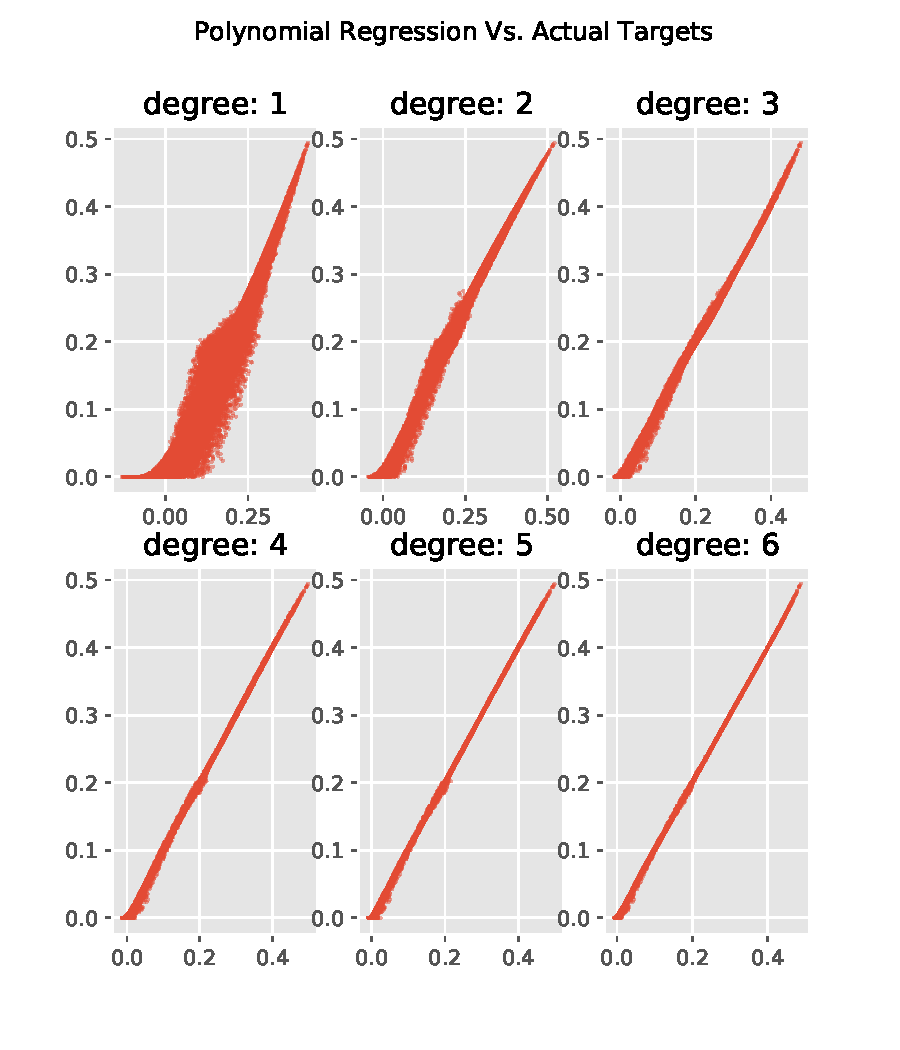
\includegraphics{Figures/polynomialEuroC.png}
\decoRule
\caption[Polynomial Regression Predictions Vs. Actual Prices]{Predicted price based on polynomial regression of varying degree}
\label{fig:PolynomialEuroC}
\end{figure}

The table is created to compare the performance for each model. The table confirms that the linear regression has a worse fit than the other models with higher capacity. The difference on the MLPs and higher order polynomial regression models less than $6\cdot 10^{-4}$ for coefficient of determination and less than $15 \cdot 10^{-3}$. The difference is negible so the fit for MLPs and polynomial regression of degree 4-6 performs all very well on the data.

\begin{table}[th]
\caption{Prediction results for european call test data for in sample polynomial regression}
\label{tab:euroPerformance}
\centering
\begin{tabular}{l l l l l l l l }
\toprule
\textbf{Model} & \textbf{Dataset} & \textbf{MSE} & \textbf{RMSE} & \textbf{MAE} & \textbf{$R^2$} \\
\midrule
Linear Reg. & In-Sample & 0.000631 & 0.025122 & 0.018264 & 0.937445\\
2. degree &  & 0.000069 & 0.008298 & 0.006136 & 0.993175\\
4. degree &  & 0.000004 & 0.002059 & 0.001282 & 0.999580\\
5. degree &  & 0.000002 & 0.001407 & 0.000864 & 0.999804\\
MLPs &  & 0.000003 & 0.001628 & 0.001337 & 0.999736\\
3. degree & In-Sample & 1.31e-05 & 0.00362470 & 0.002559 & 0.998698\\
6. degree & In-Sample & 9.23e-07 & 0.000961 & 0.000592 & 0.999908\\
MLPs & In-Sample & 0.000006 & 0.002419 & 0.001966 & 0.99942\\
\bottomrule\\
\end{tabular}
\end{table}

\subsection{Out of sample predictions}
All the models considered had good performance on the in-sample dataset except of the too simple models linear regression and 2. degree polynomial regreesion. To test the predictive strength for the models, we test the models with out-of-sample data. Specifically we consider longer maturity and deep-out-of-money options (see table \ref{tab:totalEuroParRange})
\begin{table}[H]
\caption{Parameter range}
\label{tab:totalEuroParRange}
\centering
\begin{tabular}{l l l l l l l }
\toprule
\textbf{Dataset} & \textbf{Moneyness} & \textbf{r} & \textbf{$\sigma$} & \textbf{T} \\
\midrule
In-Sample & 0.8-1.2 & 1\%-3\% & 0.05-0.5 & 1/252-3.0\\ 
Out-Of-Money & 0.6-0.8 & 1\%-3\% & 0.05-0.5 & 1/252-3.0\\ 
Longer Maturity & 0.8-1.2 & 1\%-3\% & 0.05-0.5 & 3-0-5.0\\ 
\bottomrule\\
\end{tabular}
\end{table}
The performance measures show that the polynomial regression that was performing better on the In-Sample dataset was due to overfitting, because the high order polynomial regression does perform poorly on out-of-sample data (see table \ref{tab:euroPerformanceComparision} and figure \ref{fig:PolynomialOutMoneyEuroC}). For the 5. order polynomial regression, we see a negative coefficient of determination, which means the model performs worse than the model with the mean as a horizontal line. This means the 5. order polynomial clearly have low predictive strength. 

\begin{table}[H]
\caption{Performance of predictive strength for different regression models}
\label{tab:euroPerformanceComparision}
\centering
\begin{tabular}{l l l l l l l l }
\toprule
\textbf{Model} & \textbf{Dataset} & \textbf{MSE} & \textbf{RMSE} & \textbf{MAE} & \textbf{$R^2$} \\
\midrule
Linear Reg. & In-Sample & 0.000631 & 0.025122 & 0.018264 & 0.937445\\
2. degree &  & 0.000069 & 0.008298 & 0.006136 & 0.993175\\
4. degree &  & 0.000004 & 0.002059 & 0.001282 & 0.999580\\
5. degree &  & 0.000002 & 0.001407 & 0.000864 & 0.999804\\
MLPs &  & 0.000003 & 0.001628 & 0.001337 & 0.999736\\
Linear Reg. & Out-Of-Money & 0.005772 & 0.075973 & 0.060936 & -2.377251\\
2. degree &  & 0.000767 & 0.027694 & 0.022203 & 0.551246\\
4. degree &  & 0.000944 & 0.030724 & 0.020542 & 0.447668\\
5. degree &  & 0.001812 & 0.042568 & 0.027125 & -0.060261\\
MLPs &  & 0.000005 & 0.002152 & 0.001569 & 0.997291\\
Linear Reg. & Longer Maturity & 0.002662 & 0.051593 & 0.041232 & 0.818143\\
2. degree &  & 0.001196 & 0.034577 & 0.026287 & 0.918316\\
4. degree &  & 0.003956 & 0.062894 & 0.039932 & 0.729744\\
5. degree &  & 0.012255 & 0.110702 & 0.064402 & 0.162742\\
MLPs &  & 0.000066 & 0.008138 & 0.005817 & 0.995475\\
\bottomrule\\
\end{tabular}
\end{table}

We see that the 2. degree polynomial is best on most of the performance measures for our-of-sample data. Notice based on MAE for out-of-money data the 4. degree polynomial performs better than the 2. degree polynomial, but if we look at the MSE the performance is best for the 2. degree polynomial. This is due to that the two measure weight errors in different ways, where the MSE penalize large error more than the MAE. Amoung the polynomial the 2. degree polynoial regression performs best, but gets outperformed by MLPs (see also figure \ref{fig:MLPsOutMoneyEuroC}). The MLPs has high predictive strength compared to the polynomials, because it performs well also on out-of-sample dataset. The section showed how succesfully MLPs can be used in a GBM model setup for pricing european options. The MLPs is not based on a model, it can only see data. This is promising because the MLPs could also be used for actual market data or different models to learn patterns. In the coming sections we will focus on american put options and basket options, where in the basket option case the MLPs benefit for the fact that it does not increase expontially with the dimension to maintain low error compared to polynomial regression. For the american put option the MLPs regression will only be considered, because the polynomial regression have low predictive strength for the simpler european option.

\begin{figure}[H]
\centering
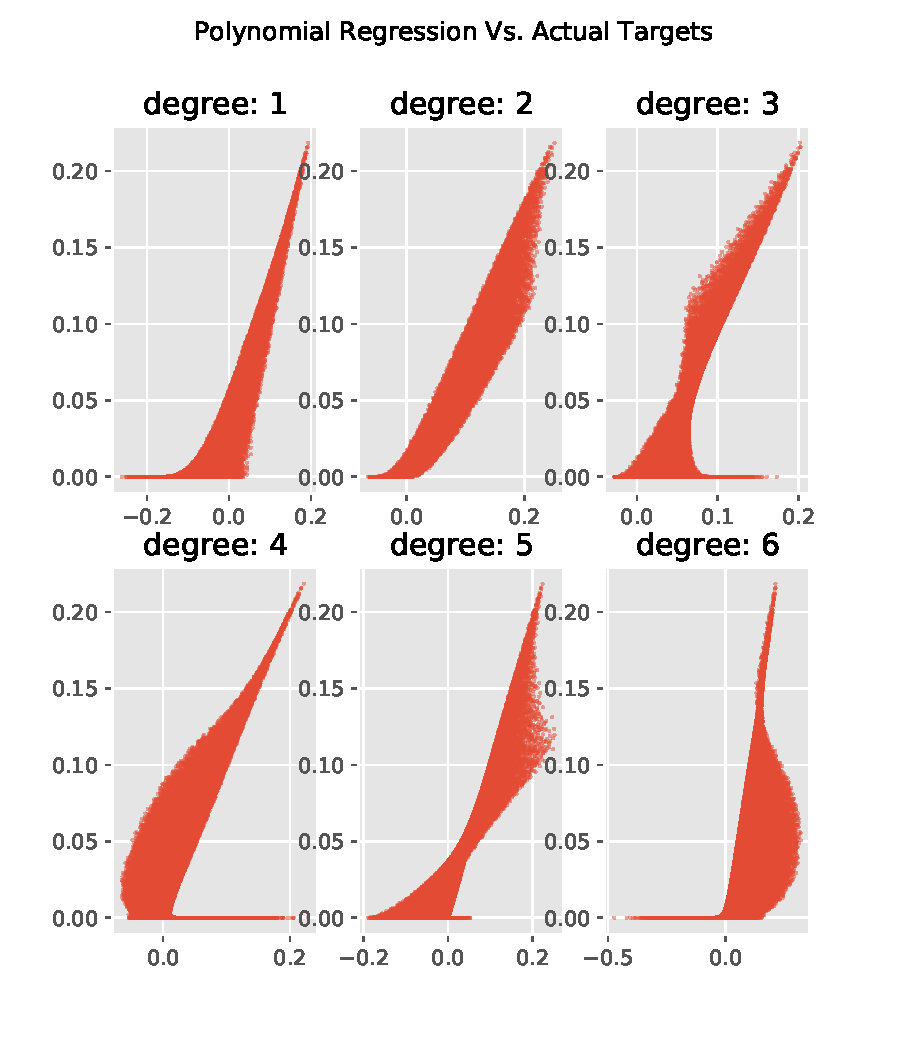
\includegraphics{Figures/polynomialOutMoneyEuroC.png}
\decoRule
\caption[Polynomial Regression Predictions Vs. Actual Prices]{Predicted price based on polynomial regression of varying degree}
\label{fig:PolynomialOutMoneyEuroC}
\end{figure}

\begin{figure}[H]
\centering
\includegraphics{Figures/PredictionOutMoneyEuroC.png}
\decoRule
\caption[MLPs Predictions Vs. Actual Prices]{Predicted price based on MLPs model}
\label{fig:MLPsOutMoneyEuroC}
\end{figure}

%\begin{figure}[th]
%\centering
%\includegraphics{Figures/PredictionLongTEuroC.png}
%\decoRule
%\caption[MLPs Predictions Vs. Actual Prices]{Predicted price based on MLPs model}
%\label{fig:MLPsEuroC}
%\end{figure}


%\begin{figure}[H]
%\centering
%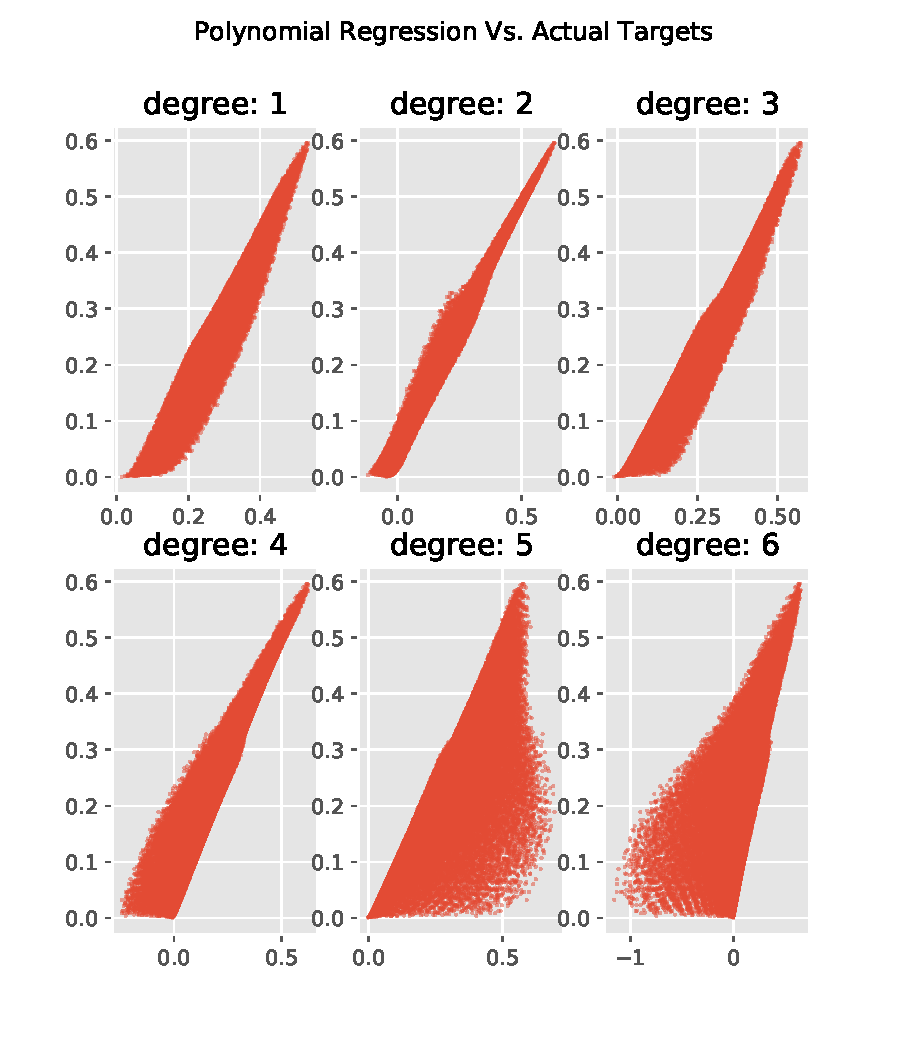
\includegraphics{Figures/polynomialLongTEuroC.png}
%\decoRule
%\caption[Polynomial Regression Predictions Vs. Actual Prices]{Predicted price based on polynomial regression of varying degree}
%\label{fig:PolynomialEuroC}
%\end{figure}


%----------------------------------------------------------------------------------------
%	SECTION 2
%----------------------------------------------------------------------------------------
\section{Multilayer Perceptrons Regression For American Options}

%-----------------------------------
%	SUBSECTION 1
%-----------------------------------
\subsection{Data}

\begin{figure}[H]
\centering
\includegraphics{Figures/marginalAmerPut.png}
\decoRule
\caption[Marginal distributions for american put]{Quasi random simulation with halton sequence}
\label{fig:marginalEuro}
\end{figure}

\begin{table}[H]
\caption{Parameter range}
\label{tab:totalEuroParRange}
\centering
\begin{tabular}{l l l l l l l }
\toprule
\textbf{Dataset} & \textbf{Moneyness} & \textbf{r} & \textbf{$\sigma$} & \textbf{T} \\
\midrule
In-Sample & 0.8-1.2 & 1\%-3\% & 0.05-0.5 & 1/252-3.0\\ 
Out-Of-Money & 1.2-1.4 & 1\%-3\% & 0.05-0.5 & 1/252-3.0\\ 
Longer Maturity & 0.8-1.2 & 1\%-3\% & 0.05-0.5 & 3-0-5.0\\ 
\bottomrule\\
\end{tabular}
\end{table}

%-----------------------------------
%	SUBSECTION 2
%-----------------------------------
\subsection{Optimization and cost function}

%-----------------------------------
%	SUBSECTION 3
%-----------------------------------
\subsection{Model Performance}

\begin{table}[H]
\caption{Performance of predictive strength for different regression models}
\label{tab:euroPerformanceComparision}
\centering
\begin{tabular}{l l l l l l l l }
\toprule
\textbf{Model} & \textbf{Dataset} & \textbf{MSE} & \textbf{RMSE} & \textbf{MAE} & \textbf{$R^2$} \\
\midrule
MLPs Reg. & In-Sample & 0.000002 & 0.001562 & 0.001278 & 0.999634\\
MLPs Reg. & Out-Of-Money & 0.000030 & 0.005503 & 0.003925 & 0.989674\\
MLPs Reg. & Longer Maturity & 0.000194 & 0.013922 & 0.010731 & 0.980759\\
\bottomrule\\
\end{tabular}
\end{table}

\begin{figure}[H]
\centering
\includegraphics{Figures/PredictionAmerP.png}
\decoRule
\caption[MLPs Predictions Vs. Actual Prices For American Put]{Predicted price based on MLPs model, where the targets are from the binomial model}
\label{fig:PredictionAmerP}
\end{figure}

\begin{figure}[H]
\centering
\includegraphics{Figures/PredictionOutMoneyAmerP.png}
\decoRule
\caption[MLPs Predictions Vs. Actual Prices For American Put]{Predicted price based on MLPs model, where the targets are from the binomial model}
\label{fig:PredictionOutMoneyAmerP}
\end{figure}

\begin{figure}[H]
\centering
\includegraphics{Figures/PredictionLongTAmerP.png}
\decoRule
\caption[MLPs Predictions Vs. Actual Prices For American Put]{Predicted price based on MLPs model, where the targets are from the binomial model}
\label{fig:PredictionOutMoneyAmerP}
\end{figure}

To compare the results by 

\begin{table}[th]
\caption{Valuation of American put option with K=40 and r=0.06.}
\label{tab:treatments}
\centering
\begin{tabular}{l l l l l l l }
\toprule
\textbf{Spot} & \textbf{$\sigma$} & \textbf{T} & \textbf{MLPs Regression} & \textbf{Binomial Tree} & \textbf{LSM} & \textbf{abs. diff.} \\
\midrule
36 & 0.2 & 1 & 4.584 & 4.488 & 4.478 & 0.010\\
36 & 0.2 & 2 & 4.649 & 4.846 & 4.828 & 0.018\\
36 & 0.4 & 1 & 7.090 & 7.119 & 7.092 & 0.027\\
36 & 0.4 & 2 & 8.487 & 8.508 & 8.500 & 0.008\\
38 & 0.2 & 1 & 3.094 & 3.260 & 3.245 & 0.015\\
38 & 0.2 & 2 & 3.638 & 3.748 & 3.735 & 0.013\\
38 & 0.4 & 1 & 6.172 & 6.165 & 6.144 & 0.021\\
38 & 0.4 & 2 & 7.605 & 7.689 & 7.665 & 0.024\\
40 & 0.2 & 1 & 2.114 & 2.316 & 2.313 & 0.003\\
40 & 0.2 & 2 & 2.779 & 2.885 & 2.881 & 0.004\\
40 & 0.4 & 1 & 5.274 & 5.310 & 5.326 & 0.016\\
40 & 0.4 & 2 & 6.839 & 6.914 & 6.908 & 0.006\\
42 & 0.2 & 1 & 1.494 & 1.622 & 1.622 & 0.000\\
42 & 0.2 & 2 & 2.167 & 2.217 & 2.212 & 0.005\\
42 & 0.4 & 1 & 4.548 & 4.602 & 4.596 & 0.006\\
42 & 0.4 & 2 & 6.197 & 6.264 & 6.243 & 0.021\\
44 & 0.2 & 1 & 1.000 & 1.117 & 1.113 & 0.004\\
44 & 0.2 & 2 & 1.678 & 1.697 & 1.688 & 0.009\\
44 & 0.4 & 1 & 3.949 & 3.956 & 3.962 & 0.006\\
44 & 0.4 & 2 & 5.649 & 5.656 & 5.649 & 0.007\\
\bottomrule\\
\end{tabular}
\end{table}


The results are promosing, because the MLPs are model free in the sense, that we could have simulated out for any model, where MLPs then learn from data only. By observing this the method can be extended to real market data in fact \parencite{GasparRaquel20} have resently showed good results for a MLPs for real market data. The next section will investigate the curse of dimensionality and the application of MLPs in this context.

%----------------------------------------------------------------------------------------
%	SECTION 3
%----------------------------------------------------------------------------------------
\section{Multilayer Perceptrons Regression For European Basket Call Max}

\parencite{FergusonRyan2018}


%----------------------------------------------------------------------------------------
%	SECTION 3
%----------------------------------------------------------------------------------------
\section{Multilayer Perceptrons Regression For Optimal Stopping}

